\section{Quantum Double Model II}
Like the toric code, we consider a lattice of local Hilbert spaces; except unlike the toric code where each on-site hilbert space was $\CC^2$ (a qubit), now the model is defined by a group $G$ with the Hilbert space at each site having dimension $\abs{G}$. There is a set of two orthnormal bases for each edge, $\set{\uparrow\ket{g}}, \set{\downarrow\ket{g}}$ where $g \in G$, with the property that flipping the direction of the arrow flips $g \to g^{-1}$. This is captured in the last figure we drew last time.

We might ask why we might not fix an orientation convention. We could do this, but it does break some symmetries in the model. So it's better to keep a ``free global'' orientation. 

\subsection{Hamiltonian for the Quantum Double Model}
We introduce two types of operators $A_g(s), B(p)$. These are related, but do not exactly coincide with the operators in the toric code.

We start with the star operator $A_g(s)$, which graphically has the action:

\begin{center}
    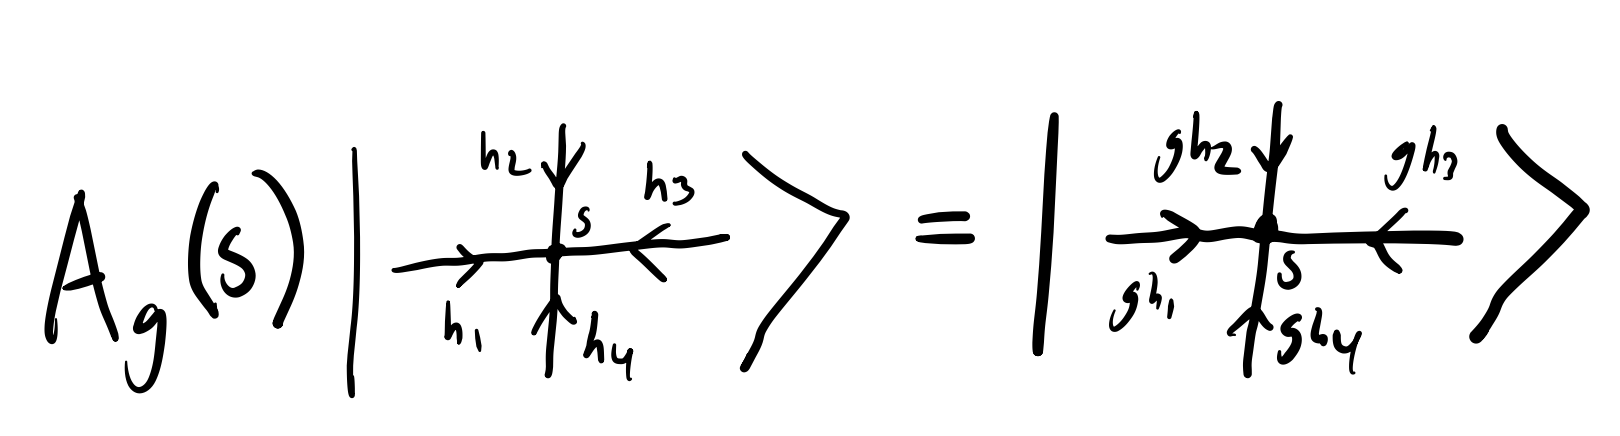
\includegraphics[scale=0.35]{Lectures/Images/lec7-Agaction.png}
\end{center}

in other words it permutes between bases elements via left-multiplication of $g$ on edges that are part of the star. It is sometimes called a ``gauge transformation''. Note that incoming arrows get left-multiplied by $g$ and outgoing arrows get right-multiplied by $g^{-1}$ (but we will derive this explicitly, we only need specify the action on incoming arrows).

The plaquette operator has the action:

\begin{center}
    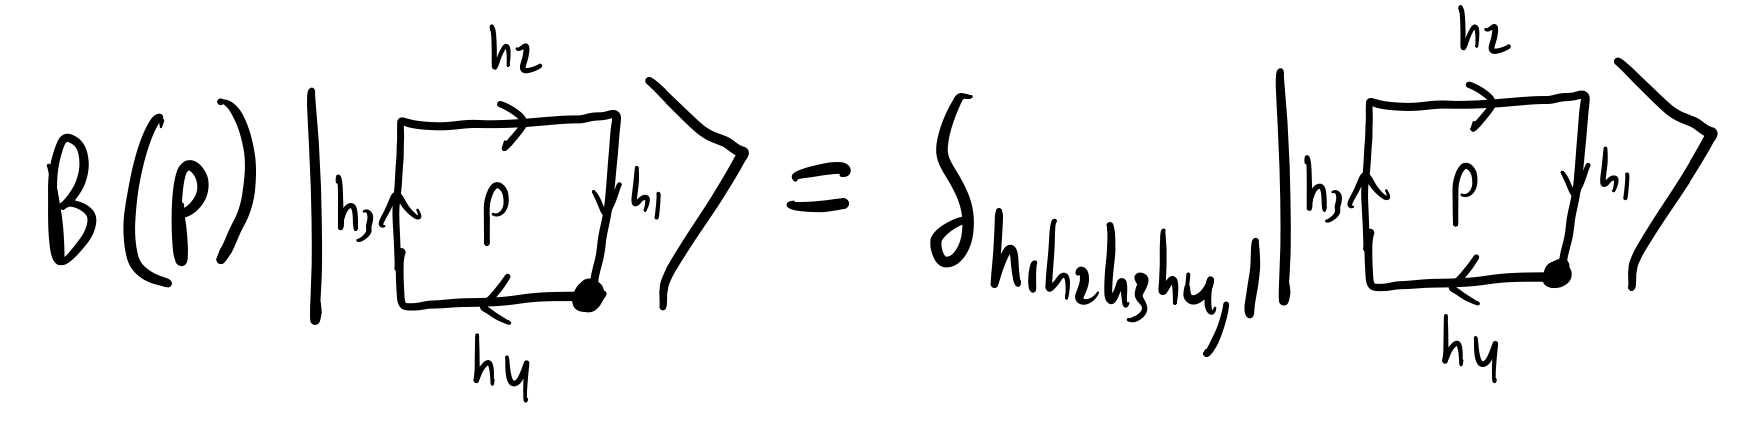
\includegraphics[scale=0.35]{Lectures/Images/lec7-Baction.png}
\end{center}

where:
\begin{equation}
    \delta_{h_1h_2h_3h_4, 1} = \begin{cases}
        1 & h_1h_2h_3h_4 = 1
        \\ 0 & \text{otherwise}
    \end{cases}
\end{equation}
The terminology we will use is that $h_1h_2h_3h_4$ is the ``flux through the plaquette $p$''.

There is a bit of convention with the multiplication of the group elements, in that we start with the basepoint in the bottom right and go around counterclockwise. We might ask that does this basepoint choice matter? If we started in the top right, we would instead get:
\begin{equation}
    h_2h_3h_4h_1 = h_1^{-1}(h_1h_2h_3h_4)h_1
\end{equation}
so concretely, different base points change flux by conjugation. But since the identity element is unchanged by conjugation, and here we only care about fluxes as identity, it will turn out to not matter here (in fact we could go in the other direction, and this changes the sign of the flux, but because the identity is self-inverse it again does not matter here. But it will matter when we look at some related operators).

Another comment; $B(p)$ are diagonal in the group element basis, while $A_g(s)$ are not. 

Now, defining the Hamiltonian in terms of these operators:
\begin{equation}
    H = - \sum_s A(s) - \sum_p B(p)
\end{equation}
where:
\begin{equation}
    A(s) = \frac{1}{\abs{G}}\sum_g A_g(s)
\end{equation}

A couple comments about this Hamiltonian. Let's check to make sure that it is indeed Hermitian. $B(p)$ is clearly Hermitian, because in our chosen orthonormal basis it is real and diagonal in the group element basis. To see that $A(s)$ is Hermitian requires a tiny bit of work. First, we notice that $A_g(s)$ is a unitary operator (because it is a permutation matrix):
\begin{equation}
    A_g(s)^\dag = A_g(s)^{-1}
\end{equation}
But since $A_g(s)$ acts via left multiplication of $g$, $A_g(s)^{-1}$ should be a left multiplication by $g^{-1}$:
\begin{equation}
    A_g(s)^\dag = A_{g}(s)^{-1} = A_{g^{-1}}(s).
\end{equation}
This tells us that in general $A_g(s)$ will not be Hermitian. But the sum will be! This is because:
\begin{equation}
    A(s)^\dag = \left(\frac{1}{\abs{G}}\sum_g A_g(s)\right)^\dag = \frac{1}{\abs{G}}\sum_{g}A_{g^{-1}}(s) = \frac{1}{\abs{G}}\sum_g A_g(s) = A(s)
\end{equation}
as the sum over all inverses of group elements is the same as the sum over all group elements.

So, the $H$ is Hermitian, and hence a valid Hamiltonian.

\subsection{Relationship to the Toric Code}
Suppose we set $G = \ZZ_2 = \set{1, g}$ with $g^2 = 1$. Then on each link we have two states; we can identify $\ket{1} \leftrightarrow \ket{Z = 1}$ and $\ket{g} \leftrightarrow \ket{Z = -1}$ with $Z$ the standard Pauli operator. We can then see what the star and plaquette operators reduce to:
\begin{equation}
    A(s) = \frac{1}{2}(A_1(s) + A_g(s)) = \frac{\II + \prod_{j \in \text{star}(s)}X_s}{2}= \frac{\II + A_s}{2}
\end{equation}
So we get the projector onto the star operator of the toric code. The same holds for $B(p)$; to have a product of group elements equal to 1 in $\ZZ_2$, this means we need an even number of $g$s. This is equivalent to projecting onto states with an even number of $Z = -1$:
\begin{equation}
    B(p) = \frac{1}{2}(\II + \prod_{j \in \partial p}Z_p) = \frac{\II + B_p}{2}
\end{equation}
which is a projection onto the toric code plaquette operator.

We thus in the $\ZZ_2$ case recover the toric code Hamiltonian (save for a bunch of identities, which doesn't affect any of the physics save for a shift in the spectrum).

\subsection{The Quantum Double Model is a Commuting Projector Hamiltonian}
We make a few claims about these operators:
\begin{enumerate}
    \item $A(s)^2 = A(s)$
    \item $B(p)^2 = B(p)$
    \item $[A(s), A(s')] = 0$
    \item $[B(p), B(p')] = 0$
    \item $[A(s), B(p)] = 0$
\end{enumerate}
Combining all of these, this tells us that $\set{A(s), B(p)}$ form a set of commuting projectors. Just like in the toric code where we had a sum of commuting operators with eigenvalues $\pm 1$, here we have a sum of commuting operators with eigenvalues $0, 1$. Let's go ahead and prove the above 5:

\begin{enumerate}
    \item We note that $A_g(s)A_h(s) = A_{gh}(s)$ which follows immediately by the definition. Then:
    \begin{equation}
        A(s)^2 = \left(\frac{1}{\abs{G}}\sum_g A_g(s)\right)\left(\frac{1}{\abs{G}}\sum_h A_h(s)\right) = \frac{1}{\abs{G}^2}\sum_{gh}A_{gh}(s)
    \end{equation}
    but now the double sum gives me every element in the group (but $\abs{G}$ different ways), thus:
    \begin{equation}
        A(s)^2 = \frac{1}{\abs{G}^2} \abs{G}\sum_g(s) = \frac{1}{\abs{G}}\sum_gA_g(s) = A(s)
    \end{equation}
    \item $B(s)^2 = B(s)$ is obvious because it has eigenvalues 1 and 0.
    \item Fix an orientation convention on the lattice where everything goes up/right.
    
    \begin{center}
        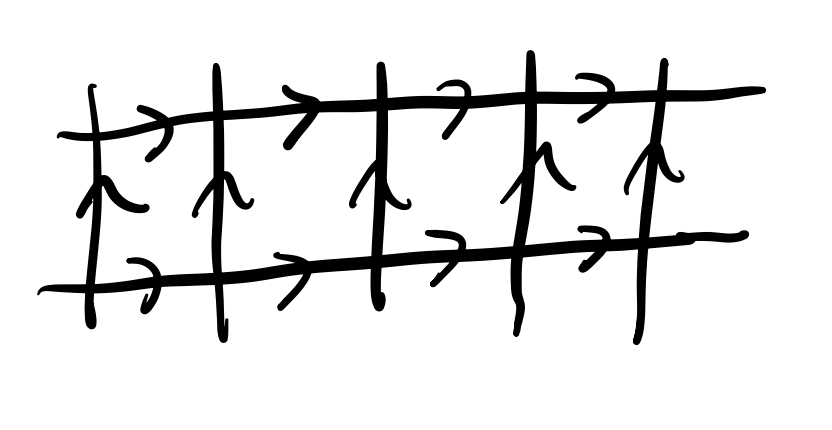
\includegraphics[scale=0.35]{Lectures/Images/lec7-orientation.png}
    \end{center}
    
    Now every star has 2 outgoing and 2 incoming arrows. So, let's work out what $A_g(s)$ in the outgoing case:

    \begin{center}
        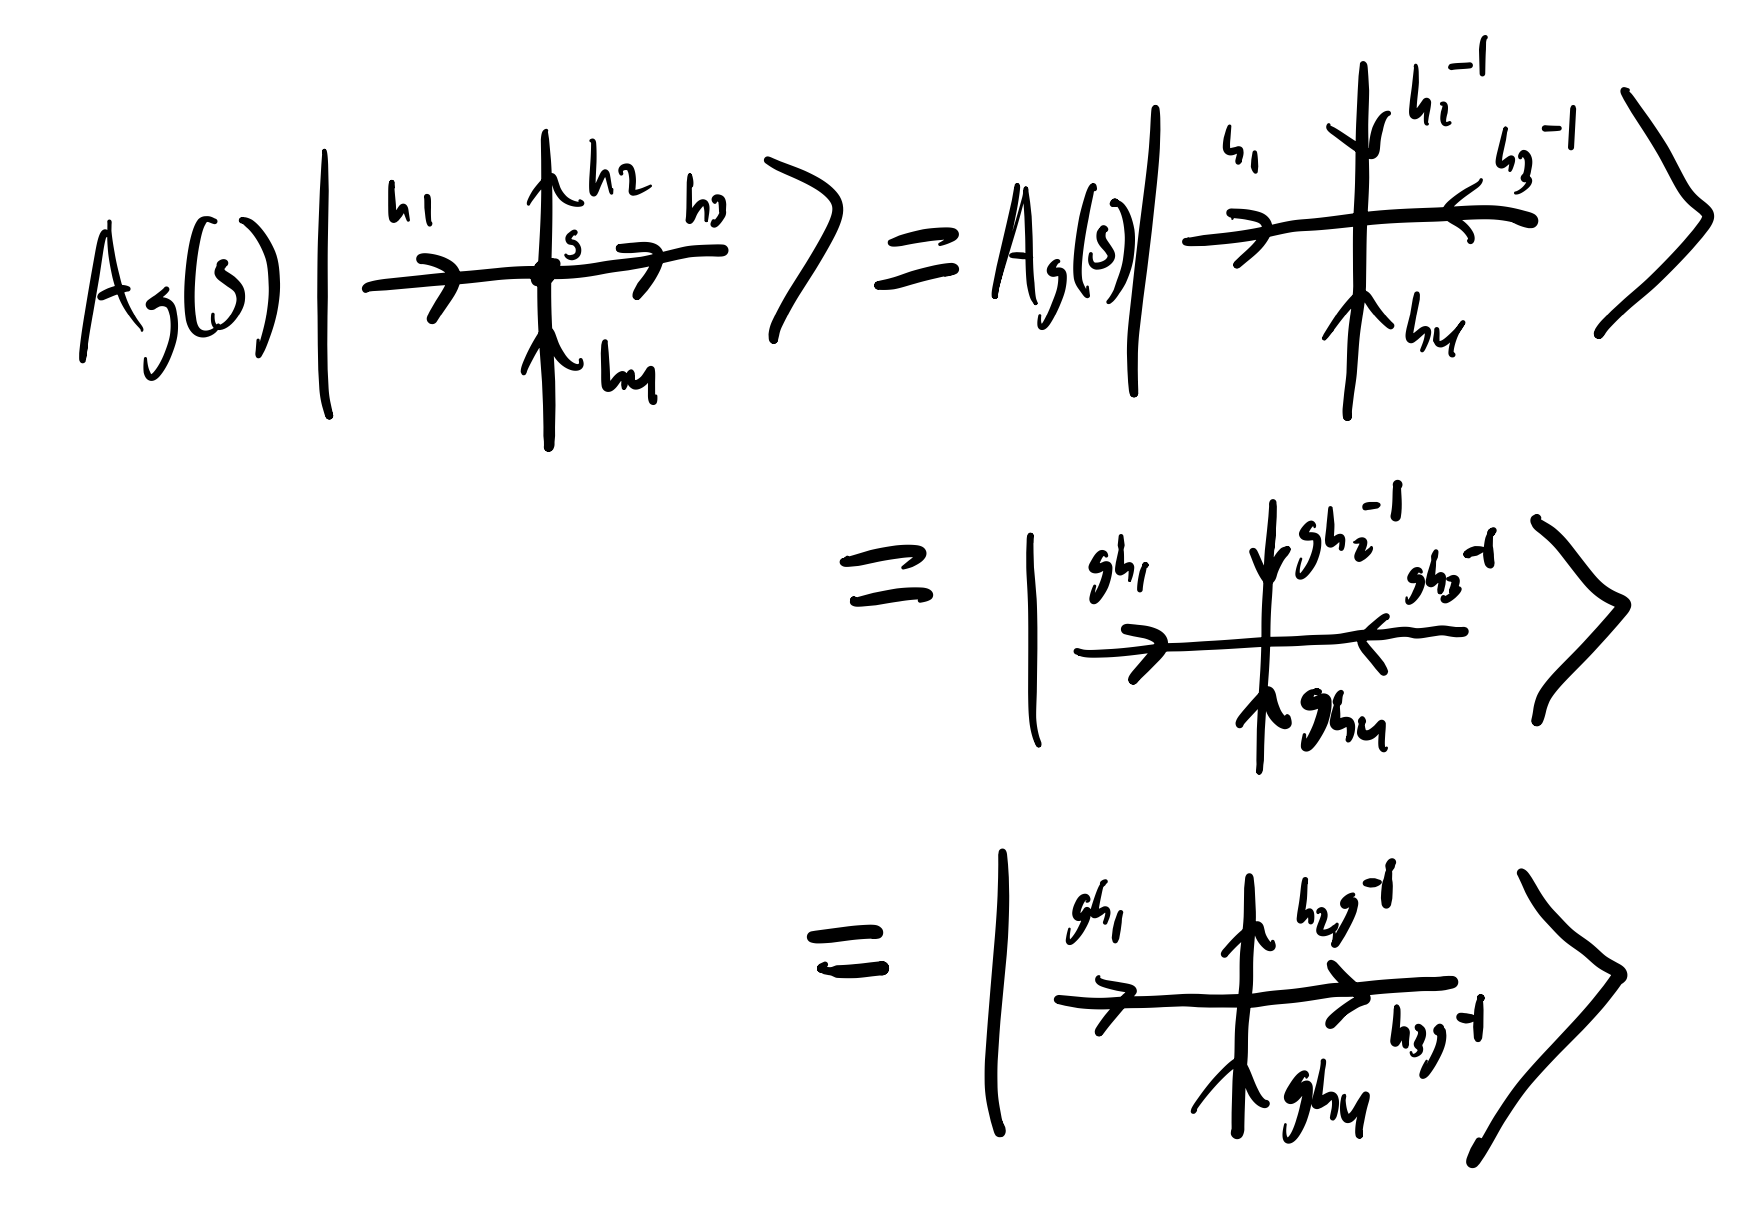
\includegraphics[scale=0.3]{Lectures/Images/lec7-Agreverse.png}
    \end{center}

    wherein in the second equality we flip the outgoing arrows so that we may apply our known action for $A_g(s)$ on incoming arrows, and in the last equality we flip again. Thus, in summary, $A_g(s)$ acts on left multiplication of $g$ on incoming arrows, and right multiplication of $g^{-1}$ on outgoing arrows.

    Now, it is easy to see that the star operators commute. We only need worry if the star operators overlap (if they don't overlap, they trivially commute):

    \begin{center}
        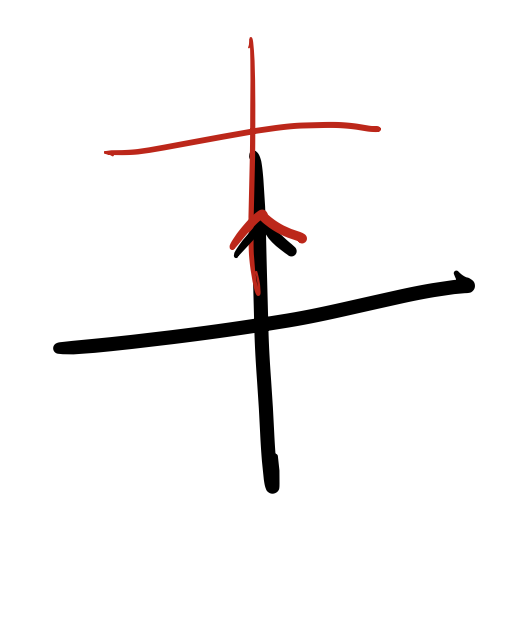
\includegraphics[scale=0.35]{Lectures/Images/lec7-staroverlap.png}
    \end{center}

    but then one will have a incoming arrow, one has an outgoing arrow (note this is true independent of any choice of orientation!). Since left and right multiplication commute, $[A_g(s), A_h(s')] = 0$ if $s \neq s'$ (if on the same site $gh \neq hg$ in general). Thus, $[A(s), A(s')] = 0$ for all $s, s'$ (the case where $s = s'$ is trivial in this case - its the same operator!)

    \item $[B(p), B(p')] = 0$ is obvious; they are all diagonal in the group element basis.
    
    \item First, we determine how to calculate the action of plaquette operator for this orientation:

    \begin{center}
        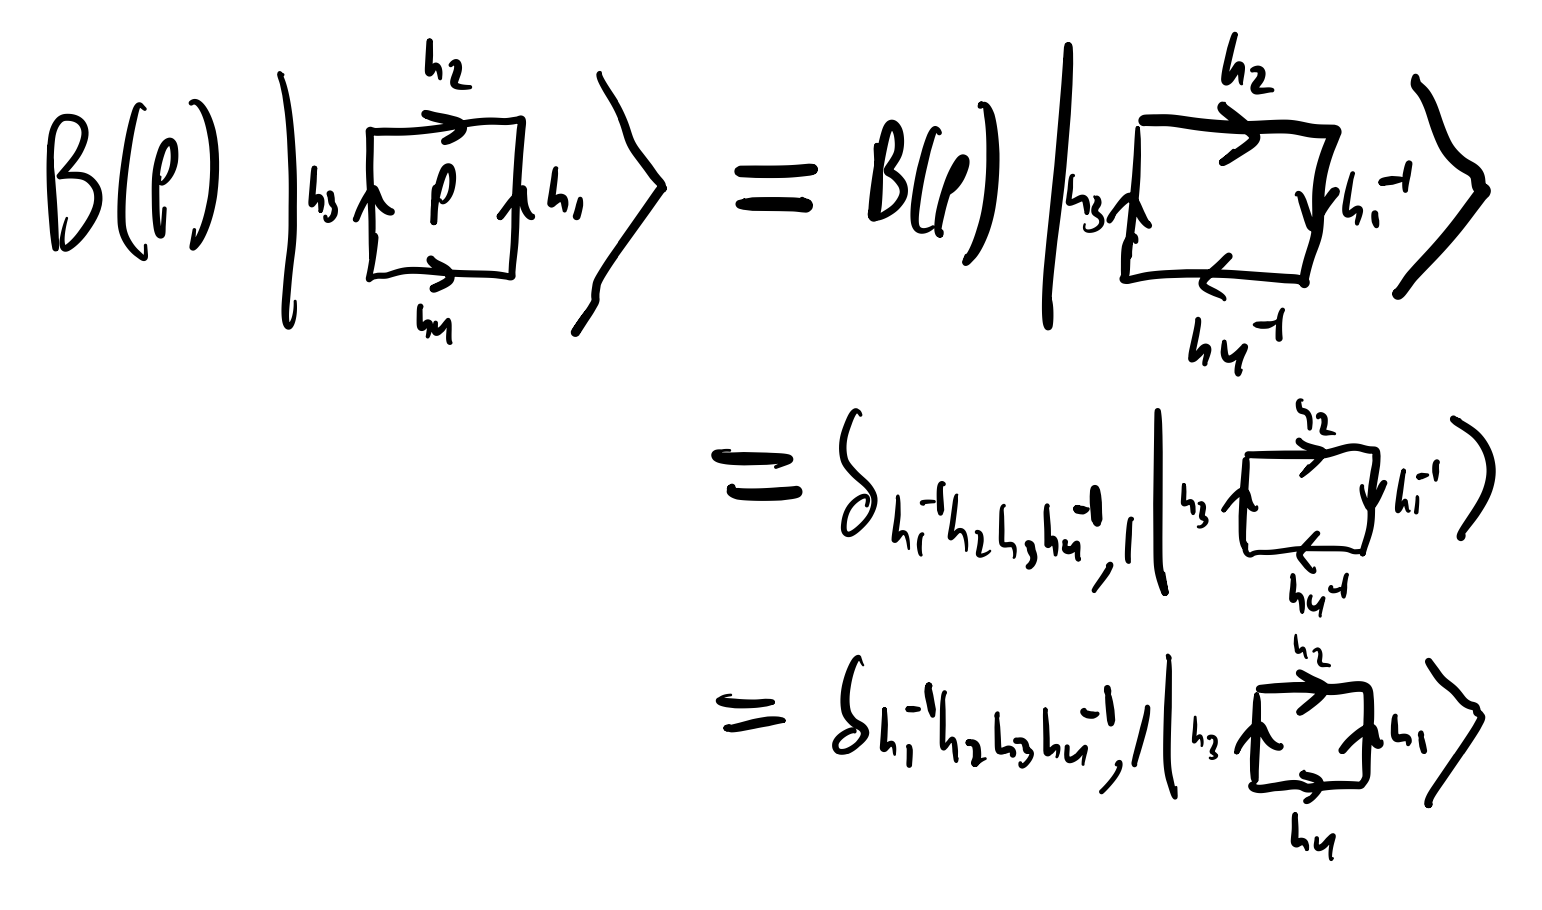
\includegraphics[scale=0.3]{Lectures/Images/lec7-Breverse.png}
    \end{center}

    where we can see if that we go against the arrow, we multiply by the inverse of the group element in the kronecker delta instead.
    
    Now for the commutation argument. If the star and plaquette have no overlap the commutation is trivial. What about when they do overlap? We have 4 cases to check. For when they overlap at the top right corner, the $A_g$ left and right multiplies in a way such that things cancel:

    \begin{center}
        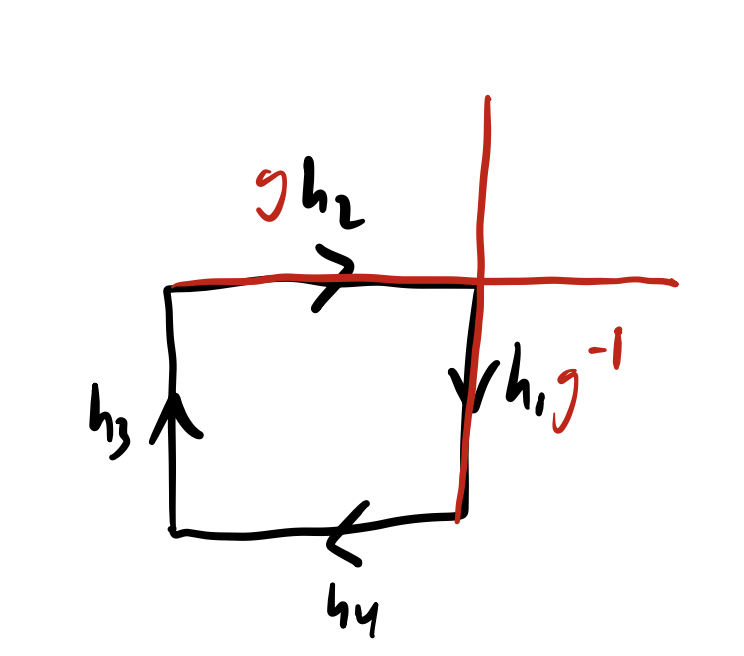
\includegraphics[scale=0.35]{Lectures/Images/lec7-overlap1.png}
    \end{center}

    \begin{equation}
        h_1h_2h_3h_4 \stackrel{A_g}{\to} (h_1g^{-1})(gh_2)h_3h_4 = h_1h_2h_3h_4
    \end{equation} 

    For the case when they overlap at the top left corner:

    \begin{center}
        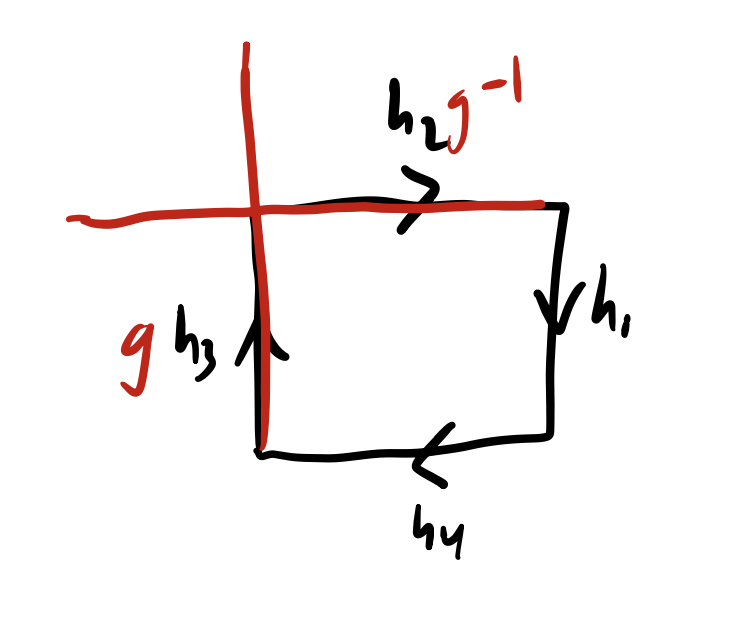
\includegraphics[scale=0.35]{Lectures/Images/lec7-overlap2.png}
    \end{center}

    \begin{equation}
        h_1h_2h_3h_4 \stackrel{A_g}{\to} h_1(h_2g^{-1})(gh_3)h_4 = h_1h_2h_3h_4
    \end{equation}

    the bottom left corner is exactly the same. The most interesting case is the bottom right corner; this is interesting case because this is our chosen basepoint from which we are measuring the flux:

    \begin{center}
        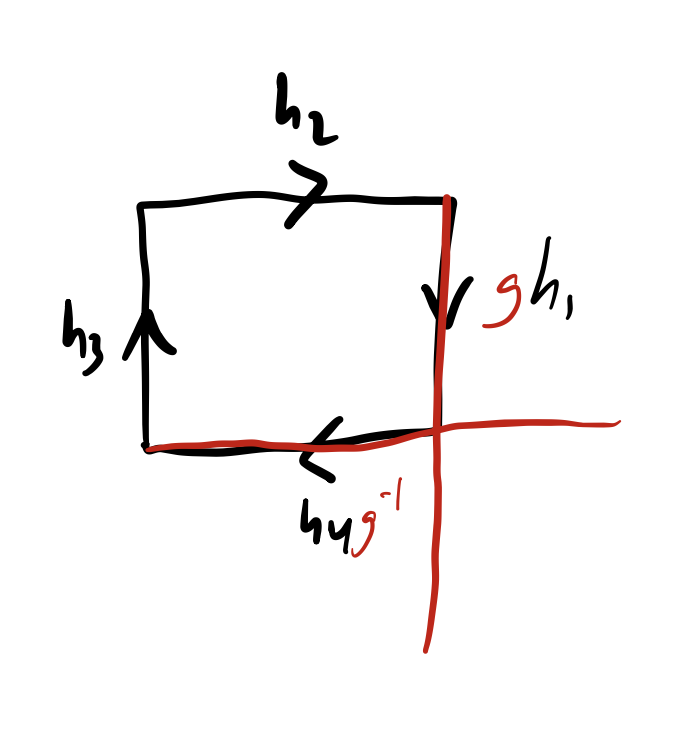
\includegraphics[scale=0.35]{Lectures/Images/lec7-overlap3.png}
    \end{center}

    \begin{equation}
        h_1h_2h_3h_4 \stackrel{A_g}{\to} (gh_1)h_2h_3(h_4g^{-1}) = g(h_1h_2h_3h_4)g^{-1}
    \end{equation}
    So $A_g$ conjugates the flux via a group element $g$ in this last interesting case. So, in all cases $A_g$ always preserves the conjugacy class of the flux $h_1h_2h_3h_4$. Thus:
    \begin{equation}
        [A_g(s), B(p)] = 0
    \end{equation}
    as 1 (and 0) are invariant under conjugation. Thus $[A(s), B(p)] = 0$.
\end{enumerate}

\subsection{Solution to the Quantum Double Model}
Since $\set{A(s), B(p)}$ are commuting projectors, i.e. have eigenvalues $0,1$, the ground states correspond to states $\ket{\Omega}$ with:
\begin{equation}
    A(s)\ket{\Omega} = B(p)\ket{\Omega} = \ket{\Omega}
\end{equation}
Our central question to answer is how many states $\ket{\Omega}$ that satisfy the above?

We consider the infinite plane geometry. From the Euler characteristic we intuit that there is a unique ground state in this case. We work in the $\ket{g}$ basis. Then:
\begin{equation}
    B(p)\ket{\Omega} = \ket{\Omega}
\end{equation}
implies that $\ket{\Omega}$ is a sum of states with ``vanishing flux'', i.e. $h_1h_2h_3h_4 = 1$. for example, on a very small lattice:

So there are many states with vanishing flux, and we can of course take linear combinations of them, so we have a linear combination with undetermined coefficients. But, we will then find that the constraint that $A(s) = 1$ everywhere enforces that all of the coefficients to be equal weight.

\begin{center}
    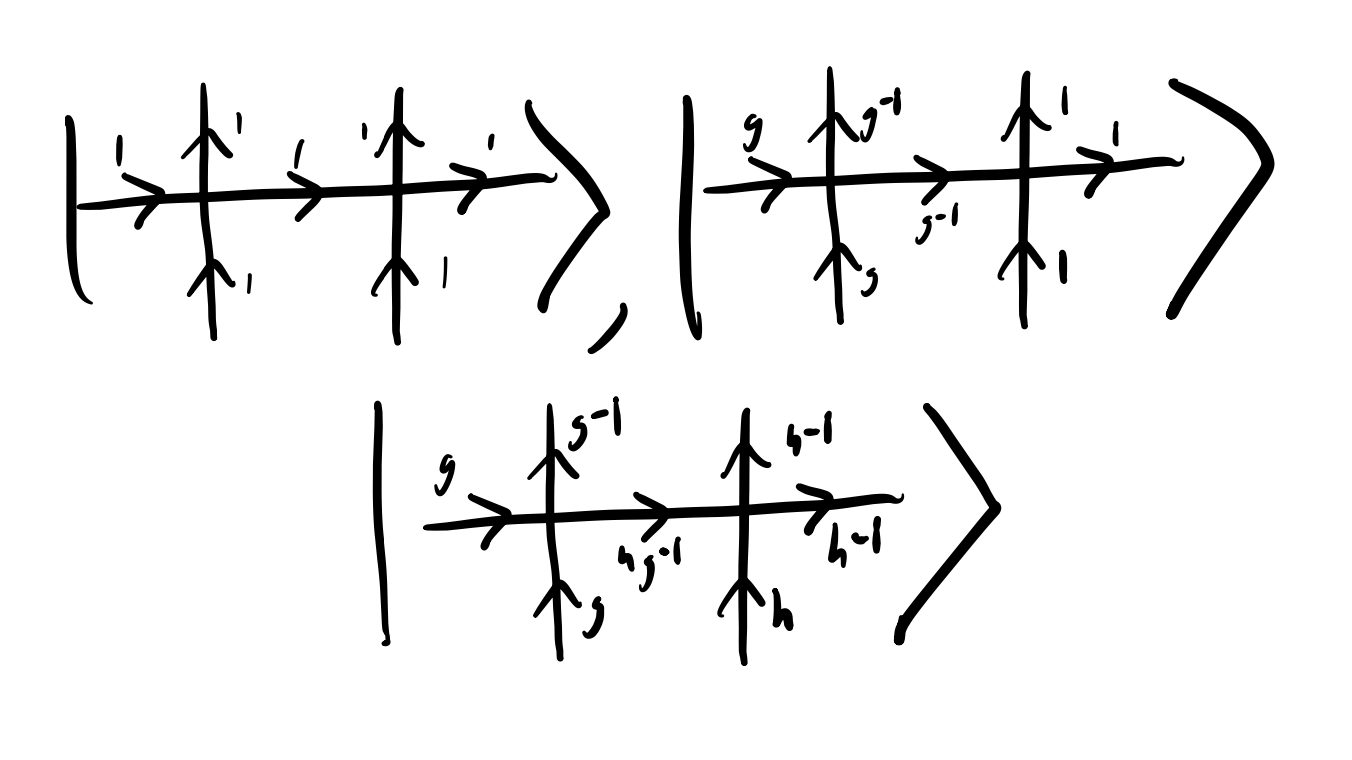
\includegraphics[scale=0.35]{Lectures/Images/lec7-nofluxstates.png}
\end{center}